\begin{figure}
	\centering
	\subcaptionbox{\label{fig:toric_code_doubling_dof}}
	{%
		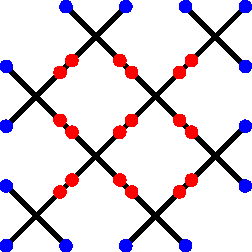
\includegraphics[scale=1]{figures/tikz/toric_code/peps_representation/peps_representation_a.pdf}
	}
	\quad
	\subcaptionbox{\label{fig:toric_code_PEPS_representation_tensor_definitions}}
	{%
		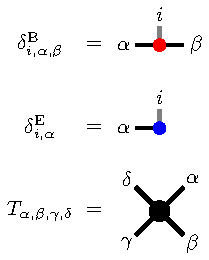
\includegraphics[scale=1]{figures/tikz/toric_code/peps_representation/peps_representation_b.pdf}
	}
	\quad
	\subcaptionbox{\label{fig:toric_code_PEPS_representation}}
	{%
		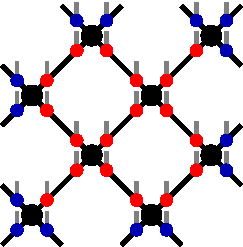
\includegraphics[scale=1]{figures/tikz/toric_code/peps_representation/peps_representation_c.pdf}
	}
	\caption{(a) To represent the Toric Code ground state as a PEPS we start by doubling the local degrees of freedom on each edge in the bulk. Bulk spins are denoted in red, while boundary spins are coloured blue. (b) Tensor diagrams of the tensors $\delta^\text{B}$, $\delta^\text{E}$ and $T$ introduced in the text. (b) The PEPS representation of the Toric Code ground state before contracting the tensors at each vertex, made up from the tensors (b).}
	\label{fig:toric_code_doubling_dof_and_PEPS_representation}
\end{figure}
\begin{figure}
	\centering
	\savebox{\largestimage}{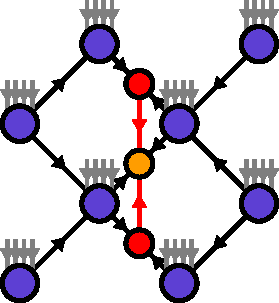
\includegraphics[scale=1]{figures/tikz/toric_code/disoTPS_representation/disoTPS_representation_a.pdf}}
	\subcaptionbox{\label{fig:toric_code_disoTPS_representation}}
	{%
		\usebox{\largestimage}
	}
	\quad\quad\quad
	\subcaptionbox{\label{fig:toric_code_disoTPS_representation_tensor_definitions}}
	{%
		\raisebox{\dimexpr.5\ht\largestimage-.5\height}
		{%
			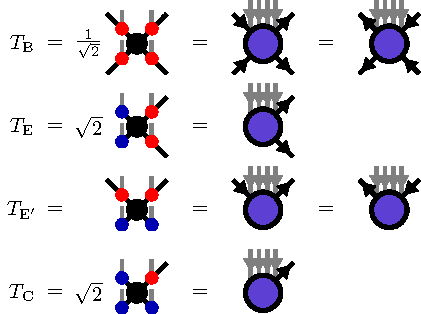
\includegraphics[scale=1]{figures/tikz/toric_code/disoTPS_representation/disoTPS_representation_b.pdf}
		}
	}
	\caption{The PEPS in figure \protect\figref{fig:toric_code_PEPS_representation} can be transformed to the disoTPS (a) by normalizing the tensors as shown in (b). Note that the tensors $T_\text{E}^\prime$ at the top and bottom edges of the lattice need a different normalization than the tensors $T_\text{E}$ at the left and right edges.}
	\label{fig:toric_code_disoTPS}
\end{figure}
We will now derive the disoTPS corresponding to the Toric Code ground state on a square lattice with open boundary condition. We choose rough boundary conditions \cite{cite:models_for_gapped_boundaries_and_domain_walls}, fixing all boundary spins to the state $\left(\ket{\uparrow} + \ket{\downarrow}\right)/\sqrt{2}$. As shown in \cite{cite:isometric_tensor_network_representation_of_string_net_liquids}, the Toric Code ground state can be represented exactly as a PEPS with bond dimension $D = 2$. One can construct such a PEPS easily by first doubling the Hilbert space on each edge as $\ket{s_i} \rightarrow \ket{s_i}\otimes\ket{s_i}$, which we show in Figure \figref{fig:toric_code_doubling_dof}. In the PEPS representation the physical degrees of freedom on each edge in the bulk are then carried by two identical tensors $\delta^\text{B}\in\mathbb{R}^{2\times2\times2}$,
\begin{equation}
	\delta^\text{B}{i,\alpha,\beta} = \begin{cases}
		1 &\text{if }i=\alpha=\beta\\
		0 &\text{else}
	\end{cases},
\end{equation}
as shown in Figure \figref{fig:toric_code_PEPS_representation_tensor_definitions}. The boundary spins are represented by tensors $\delta_E\in\mathbb{R}^{2\times2}$,
\begin{equation}
	\delta^\text{E}{i,\alpha} = \begin{cases}
		1 &\text{if }i=\alpha\\
		0 &\text{else}
	\end{cases}.
\end{equation}
We proceed by associating each vertex with the spins on the four connected edges and connect the corresponding tensors $\delta^\text{B}$ and $\delta^\text{E}$ with a tensor $T\in\mathbb{R}^{2\times2\times2\times2}$ that is placed on each vertex,
\begin{equation}
	T_{i,j,k,l} = \begin{cases}
		1 & \text{if } \left(i+j+k+l\right)\mod2 = 0 \\
		0 & \text{else}
	\end{cases}.
\end{equation}
This tensor ensures that all states with an odd number of down spins around a vertex have an amplitude of zero, satisfying condition \eqref{eq:toric_code_A_operator_condition}. \par
We arrive at the PEPS in Figure \figref{fig:toric_code_PEPS_representation}. Each basis state satisfying condition \eqref{eq:toric_code_A_operator_condition} results in the same amplitude when contracting the PEPS, while basis states violating the condition vanish. Thus, the PEPS represents the ground state of the Toric Code. \par
We now want to transform the PEPS into a disoTPS. This can be easily done by choosing the correct normalization for the vertex tensors, which transforms them into isometries as shown in Figure \figref{fig:toric_code_disoTPS_representation_tensor_definitions}. Note that different normalizations need to be chosen for tensors at the corners, edges, and in the bulk. For each vertex tensor we can choose the isometry direction to point to the left or to the right respectively, allowing us to place the orthogonality hypersurface anywhere in the lattice. As a last step, the tensors of the orthogonality hypersurface must be specified. The two spins that are connected to a tensor $W$ of the orthogonality hypersurface must be in the same local state, since they were created by doubling the local degree of freedom. This constraint can be enforced by setting $W\in\mathbb{R}^{2\times1\times2\times1}$ to
\begin{equation}
	W_{\alpha,\nu,\beta,\mu} = \frac{\delta_{\alpha,\beta}}{\sqrt{2}}
\end{equation} 
with dummy indices $\nu, \mu$ of bond dimension $1$. Trivially, the tensors $W$ fulfil the isometry condition. We can again choose the direction of isometry to point either up or down for every $W$-tensor, allowing us to place the orthogonality center freely along the orthogonality hypersurface.\par
We have thus found an exact disoTPS representation of the Toric Code ground state with $D = 2$ and $\chi= 1$, similar to the construction done in \cite{cite:isometric_tensor_network_representation_of_string_net_liquids} for isoTPS. The final network is depicted in Figure \figref{fig:toric_code_disoTPS_representation}. We test the different algorithms for the YB move on the Toric Code ground state on a $5\times5$ lattice. All algorithms are able to move the orthogonality surface exactly up to computational accuracy. This however only works well if a good initialization is chosen for the disentangling unitary. We choose an initialization based on an SVD, see \cite{cite:isometric_tensor_network_states_in_two_dimensions, cite:efficient_simulation_of_dynamics_in_two_dimensional_quantum_spin_systems} or our implementation \cite{cite:github_disoTPS}.